\documentclass[11pt]{hcmut-report}
\usepackage{codespace}
\usepackage{amssymb}
\usepackage{caption}
\usepackage{subcaption}
\usepackage{array}
\usepackage{longtable}
\usepackage{caption}
\usepackage{listings}
\usepackage{tikz}
\usepackage{hyperref}
\usepackage{minted} % for minted code
% Encodings
\usepackage{gensymb, textcomp}
% Better tables
% Wide tables go to https://tex.stackexchange.com/q/332902
\usepackage{array, multicol, multirow, siunitx, tabularx}
\usepackage{blindtext}
% Better enum
\usepackage{enumitem}
% Graphics
\usepackage{caption, float}
\usepackage{subcaption}

\DeclareCaptionFormat{custom} {
    \textbf{#1#2}\textit{\small #3}
}
\captionsetup{format=custom}

\usepackage[export]{adjustbox}

% For demonstration purposes, remove in production
\usepackage{mwe}

% % Configurations
\newcounter{memberrowno}
\setcounter{memberrowno}{0}
\reportlayout%

% Override (some) default values
\ocoursename{COMPUTER ARCHITECTURE (CO2007)}
\oreporttype{Computer Architecture Assignment - Semester 232}
\title{CALCULATOR}
\oadvisor{MSc. Nguyễn Thiên Ân}

% Custom commands
\newcommand*\mean[1]{\bar{#1}}

\begin{document}
    \coverpage%
    
    \newpage
        \tableofcontents
    \newpage
        \listoffigures
        \listoftables
    \newpage
    
    \nocite{*}
    
    \setcounter{section}{-1}
    \section{Abstraction}
        
This report encapsulates the design, development, and evaluation of the MIPS32 assembly program that emulates a versatile calculator[\ref{fig:CasioCalculator}]. The program's core functionalities encompass basic arithmetic operations, error handling, memory management, and log file generation. Users can input mathematical expressions through a user-friendly interface, receiving accurate results promptly. The calculator supports arithmetic operations such as \emph{addition}, \emph{subtraction}, \emph{multiplication}, and \emph{division}, along with advanced functions like \emph{factorization} and \emph{exponentiation}. Error detection mechanisms ensure the integrity of user input, while \emph{memory functionality} stores the last result for reuse. Decimal numbers are handled with precision, and a comprehensive \emph{log file} captures user interactions and calculated outcomes for future reference. 

\begin{figure}[htbp]
  \centering
  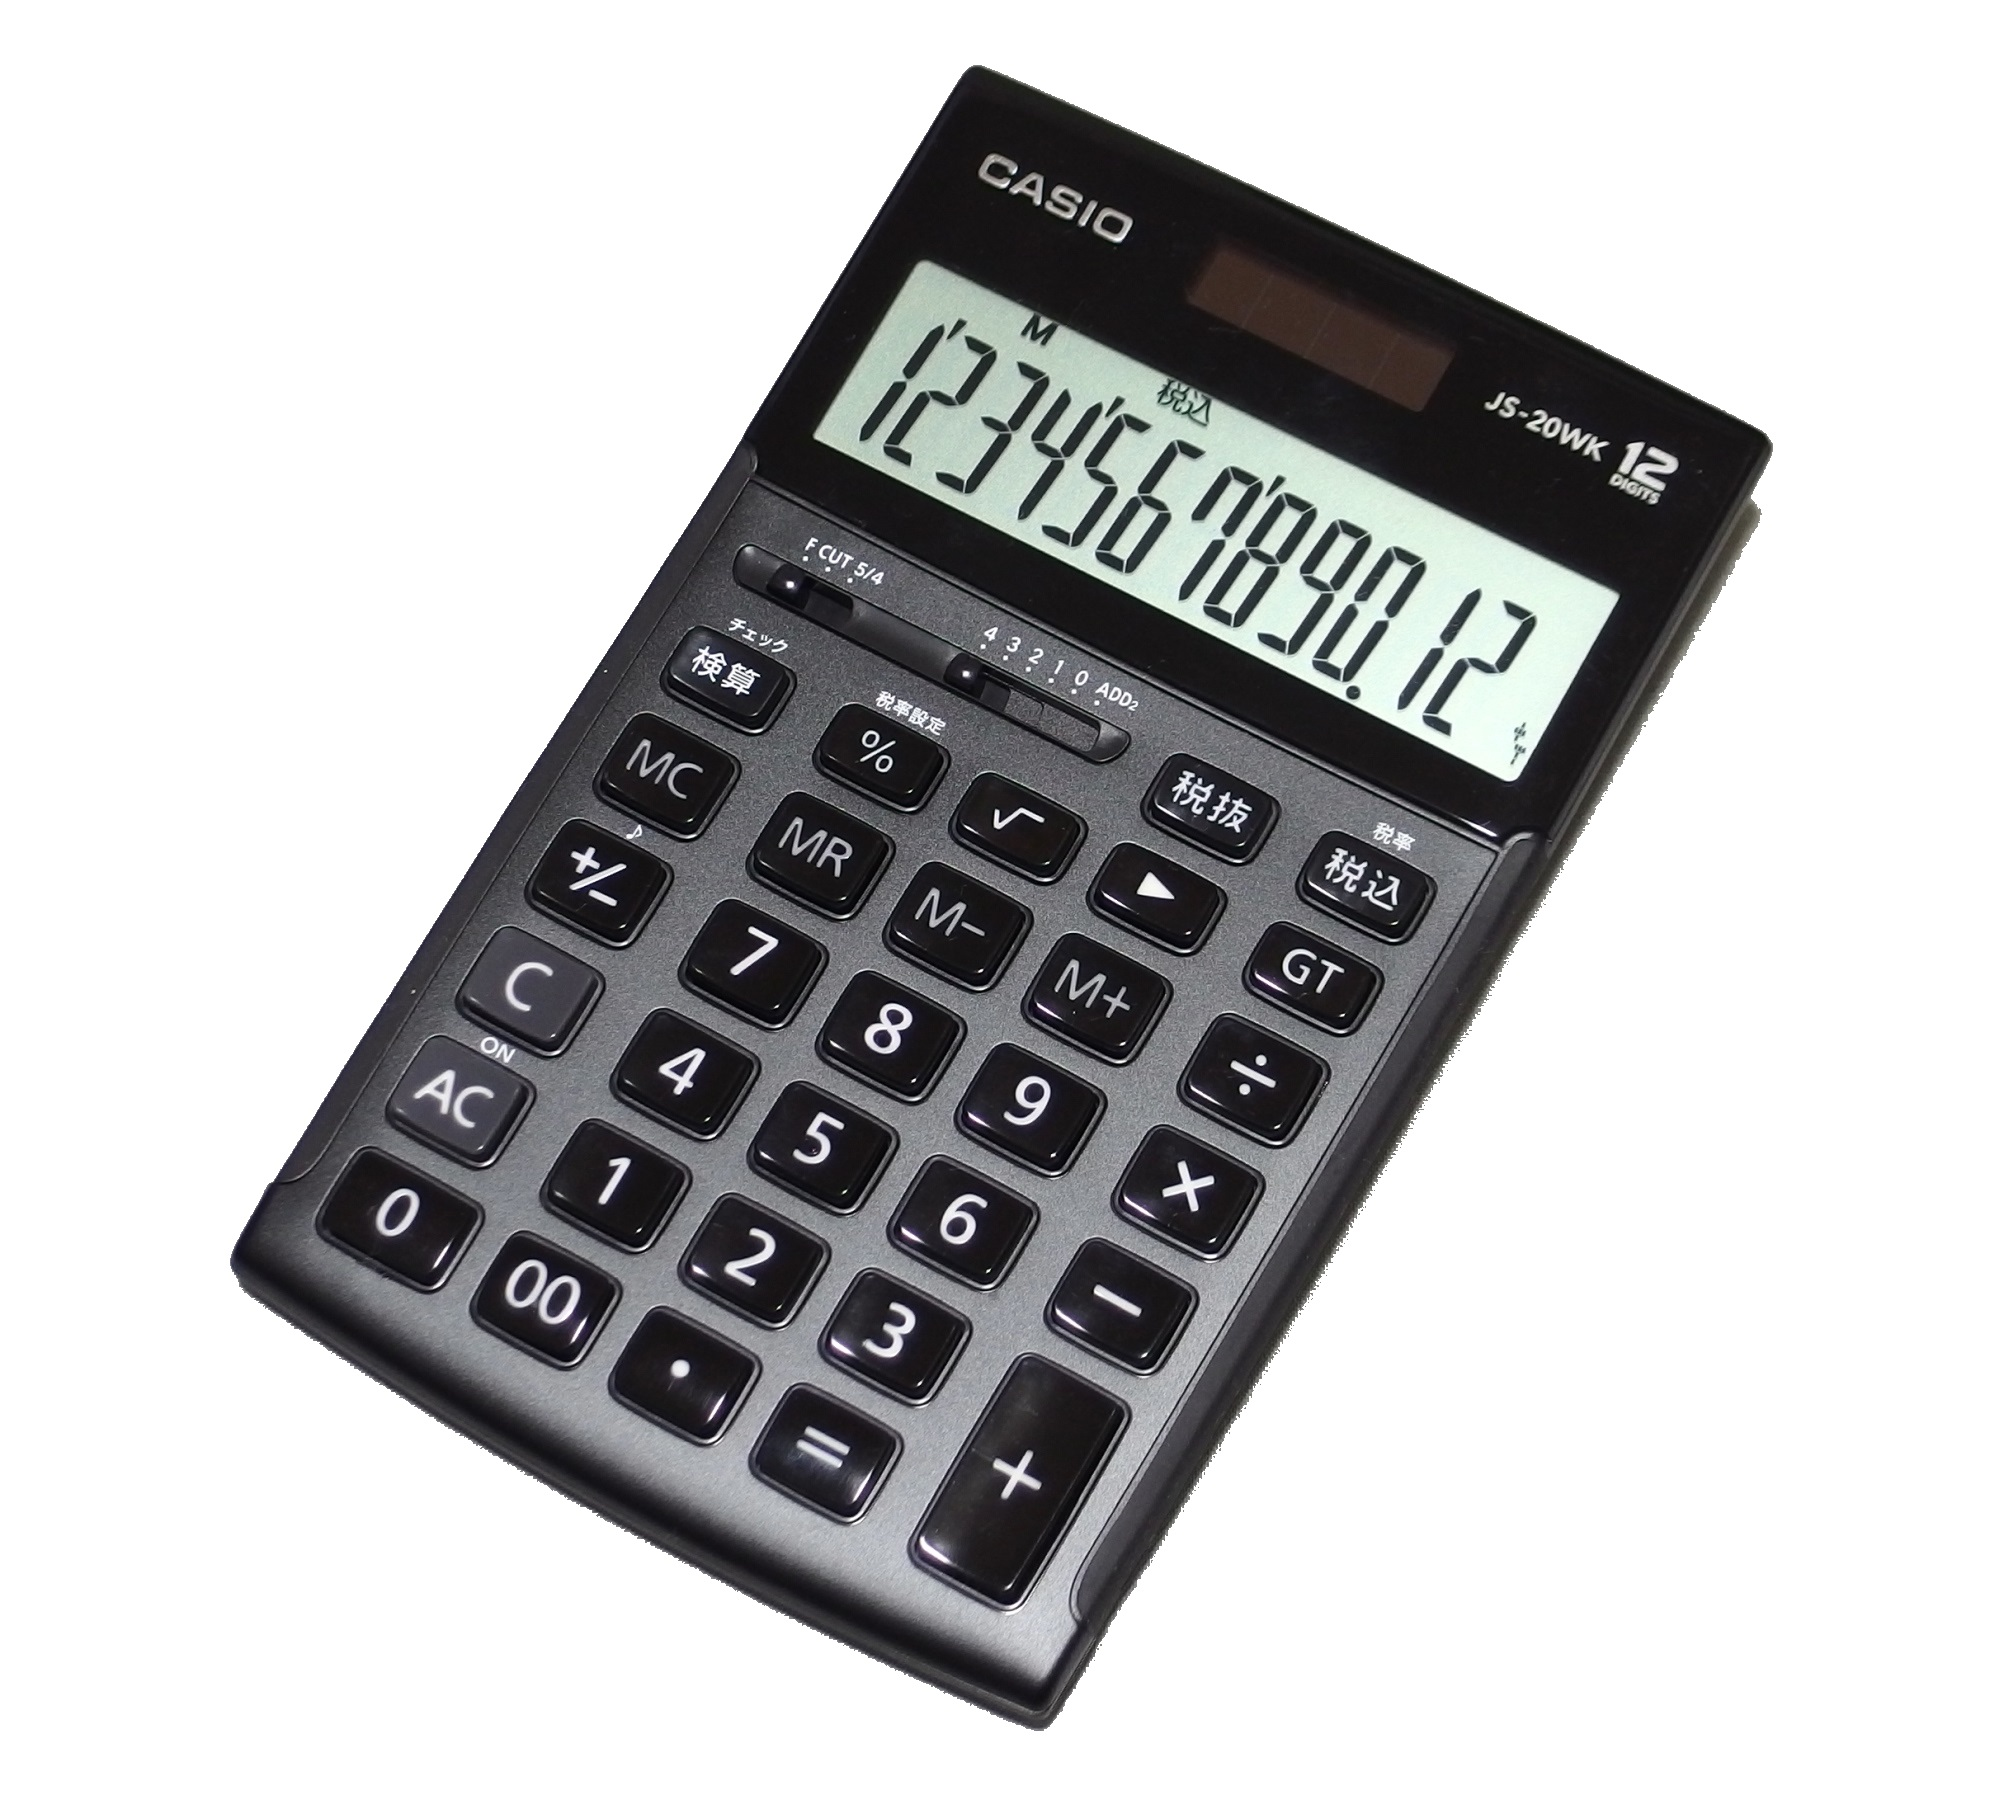
\includegraphics[width=0.7\textwidth]{graphics/0.CasioCalculator.jpg}
  \caption{Casio calculator}
  \label{fig:CasioCalculator}
\end{figure}

The report delves into the \textbf{algorithmic strategies} employed, the \textbf{methodologies of implementation}, and the \textbf{limitations} inherent to this program.
Visual aids such as flowcharts and test case outcomes supplement the narrative, providing clarity and insight into the program's inner workings. The submission adheres rigorously to the evaluation rubric, emphasizing interface friendliness, application functionality, and the quality of the accompanying report. Plagiarism concerns are addressed through originality and adherence to academic integrity standards, ensuring the integrity of the submitted work.
    \section{User Guide and Application Interface}
\label{sec:1.Guide&Interface}

\subsection{Run On Terminal}
\label{sec:1.Terminal}
    This program uses ANSII color codes for display, so it is recommended to run it on Terminal rather than \texttt{Mars45} software [\ref{sec:1.Mars45}] for the best experience. To run it on the terminal, use the following command:
    
    \begin{code}{Python}
        >>> spim mar.asm
    \end{code}
    \begin{lstlisting}[language=bash, caption={Running the program on Terminal}]
    \end{lstlisting}
    
    After using the above command, there will be a vibrant and user-friendly colored frame providing usage instructions [\ref{fig:1.InitProgram}]. Information in the frame includes the author, last updated date, input instructions, and some notes.
    
    \begin{figure}[htbp]
        \centering
        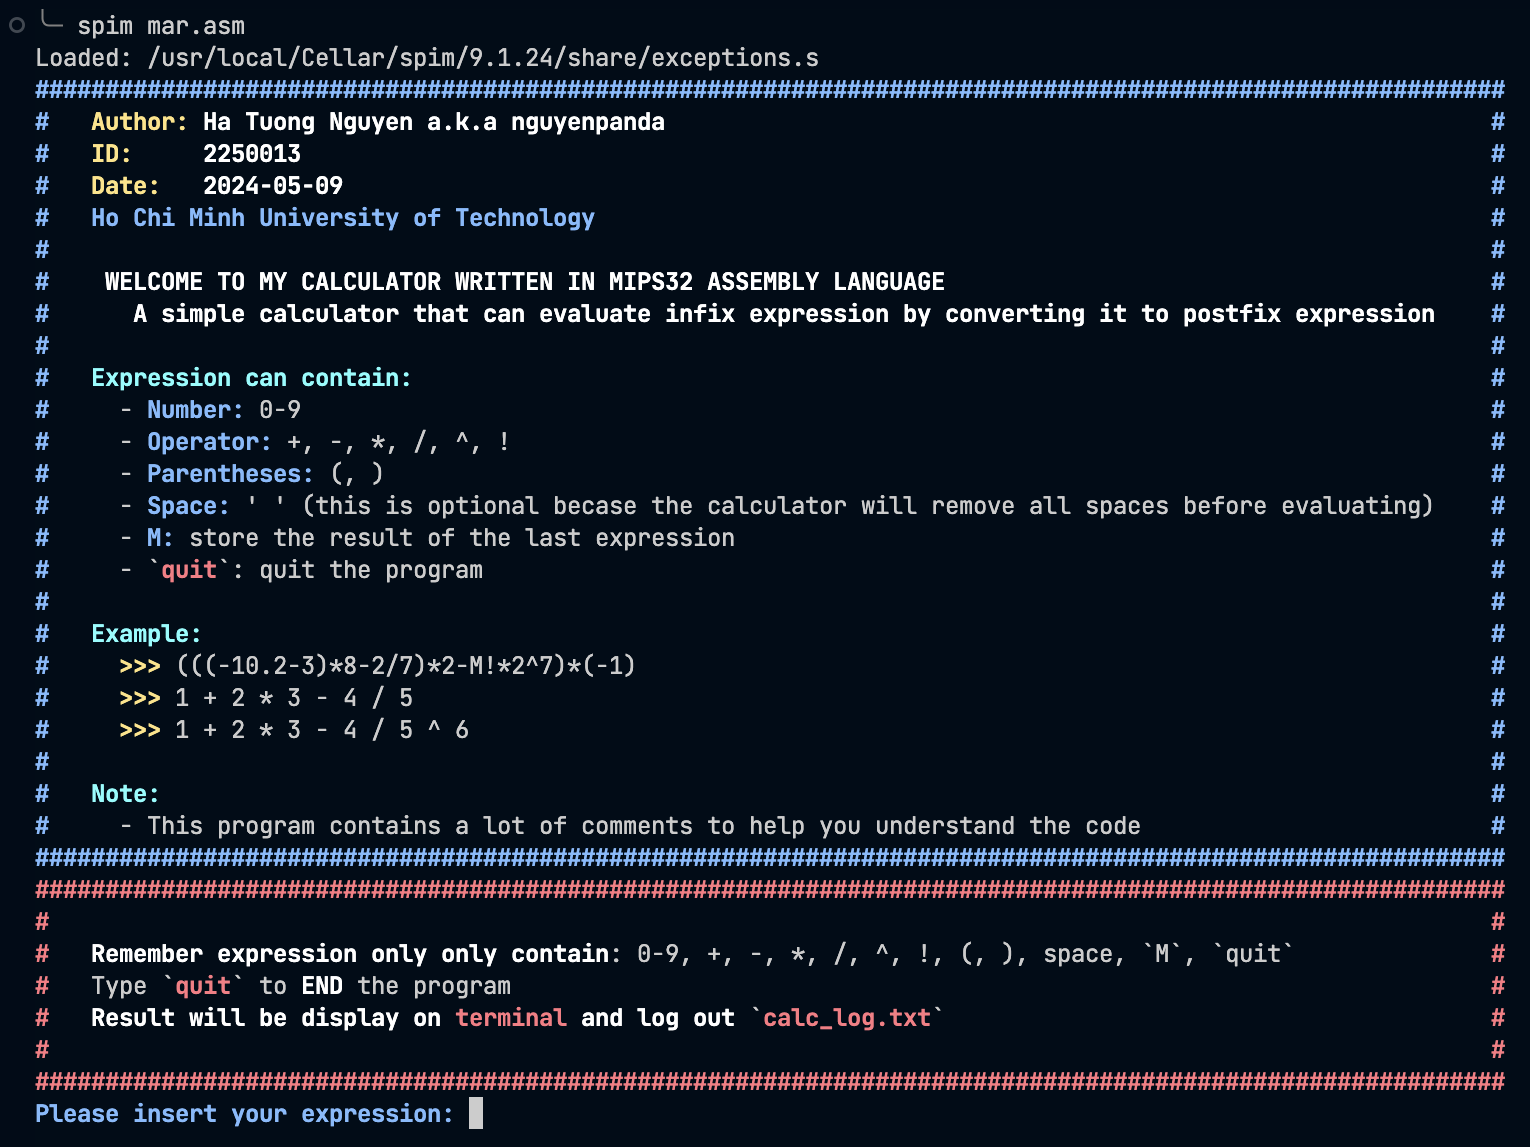
\includegraphics[width=1\textwidth]{graphics/1.Init.png}
        \caption{Starting the program}
        \label{fig:1.InitProgram}
    \end{figure}
    
    When entering an expression and pressing enter, the software will calculate and display the result of the operation. Simultaneously, it will display a red instruction frame for the next steps for the user. Meanwhile, the value of that operation will be saved in '\texttt{M}' and written to the file '\texttt{calc\_log.txt}' with \emph{16 decimal places} after the decimal point.
    
    \begin{figure}[htbp]
        \centering
        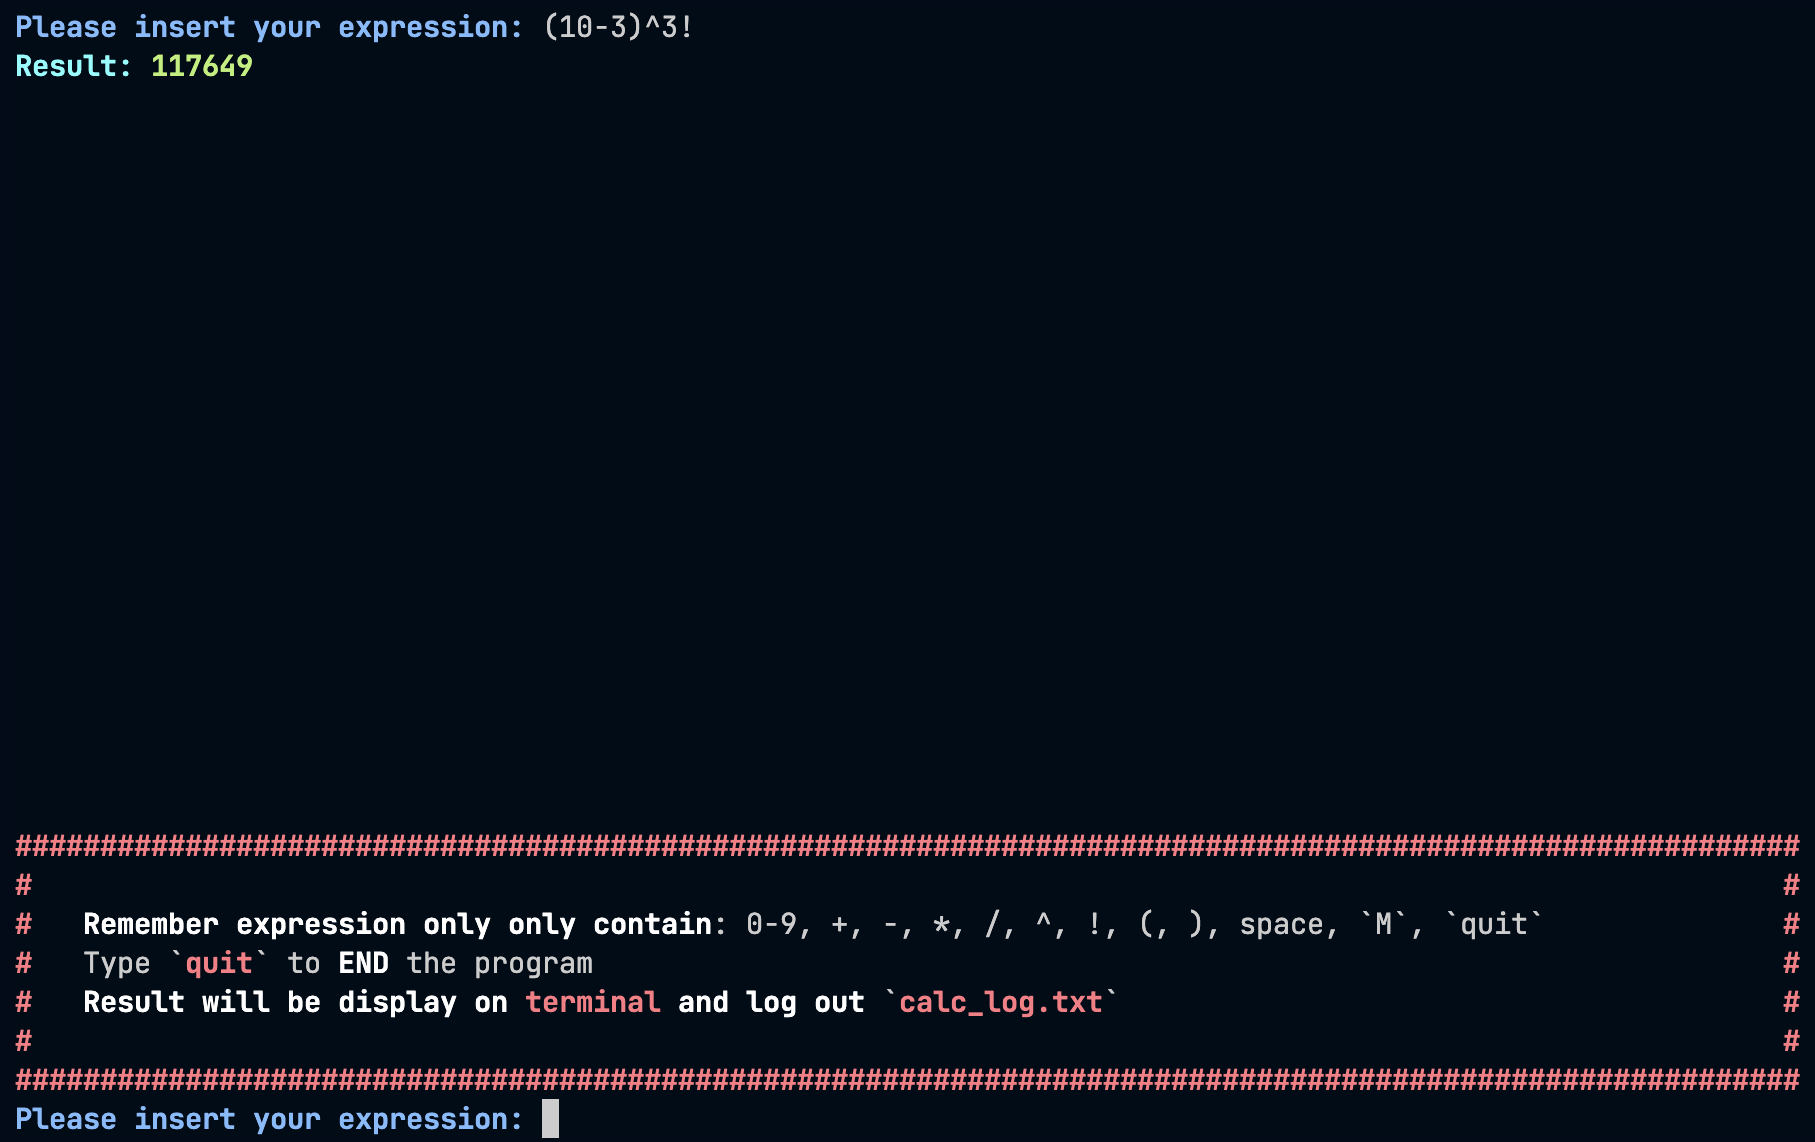
\includegraphics[width=1\textwidth]{graphics/1.AfterCalculate.png}
        \caption{After entering the first expression}
        \label{fig:1.AfterCalculate}
    \end{figure}
    
    If the user enters '\texttt{quit}', the program will terminate and notify the user that they have entered '\texttt{quit}', ending the program.
    
    \begin{figure}[htbp]
      \centering
      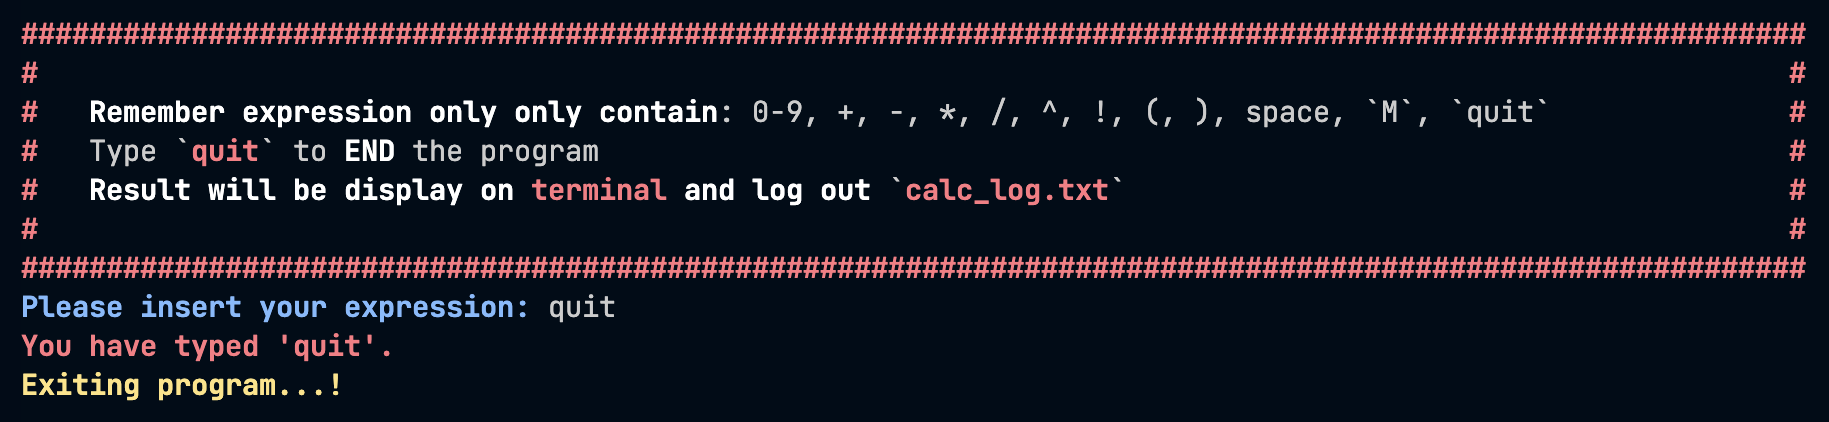
\includegraphics[width=1\textwidth]{graphics/1.Quit.png}
      \caption{User enter '\texttt{quit}'}
      \label{fig:1.EnterQuit}
    \end{figure}

\subsection{Run On Mars45}
\label{sec:1.Mars45}

    If you prefer not to run it on the terminal, you can run it on \textit{Mars45}. This is done very simply by downloading the \textit{Mars45} software from this link [\href{https://courses.missouristate.edu/kenvollmar/mars/download.htm}{Missouri State University}]. After downloading, open the file and then click \texttt{Assemble} \(\rightarrow\) \texttt{Run}.

    \begin{figure}[htbp]
        \centering
        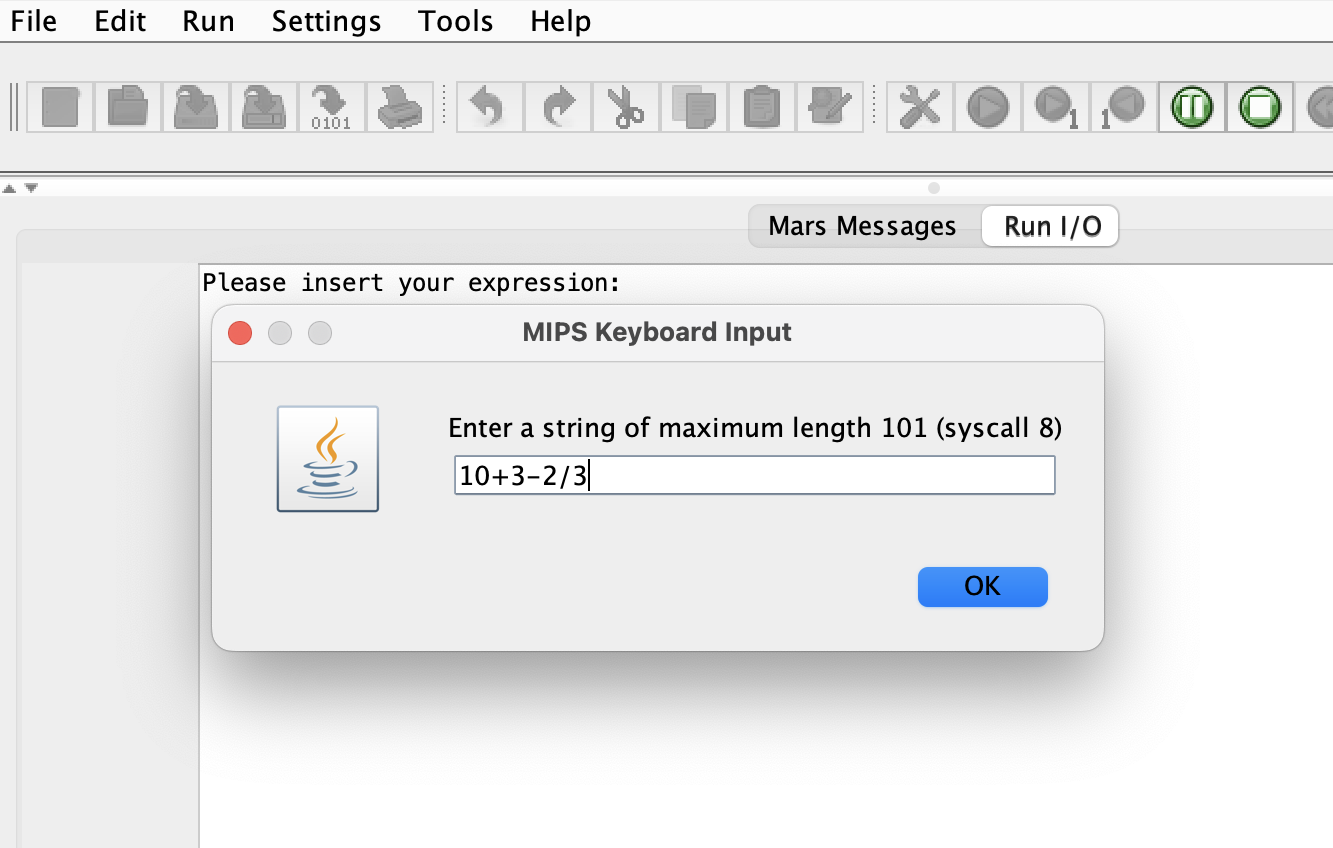
\includegraphics[width=0.6\textwidth]{graphics/1.Mars45Enter.png}
        \caption{Starting the program on \textit{Mars45}}
        \label{fig:1.MarsEnter}
    \end{figure}

    However, using \textit{Mars45} will not display the vibrant colored instruction frame because \textit{Mars45} does not support ANSII color-coded character output. This can be easily overcome by going to Settings and enabling '\texttt{Popup dialog for input syscalls}'. When running, you will see a dialog box and the result on '\texttt{Run I/O}'.

    \begin{figure}[htbp]
        \centering
        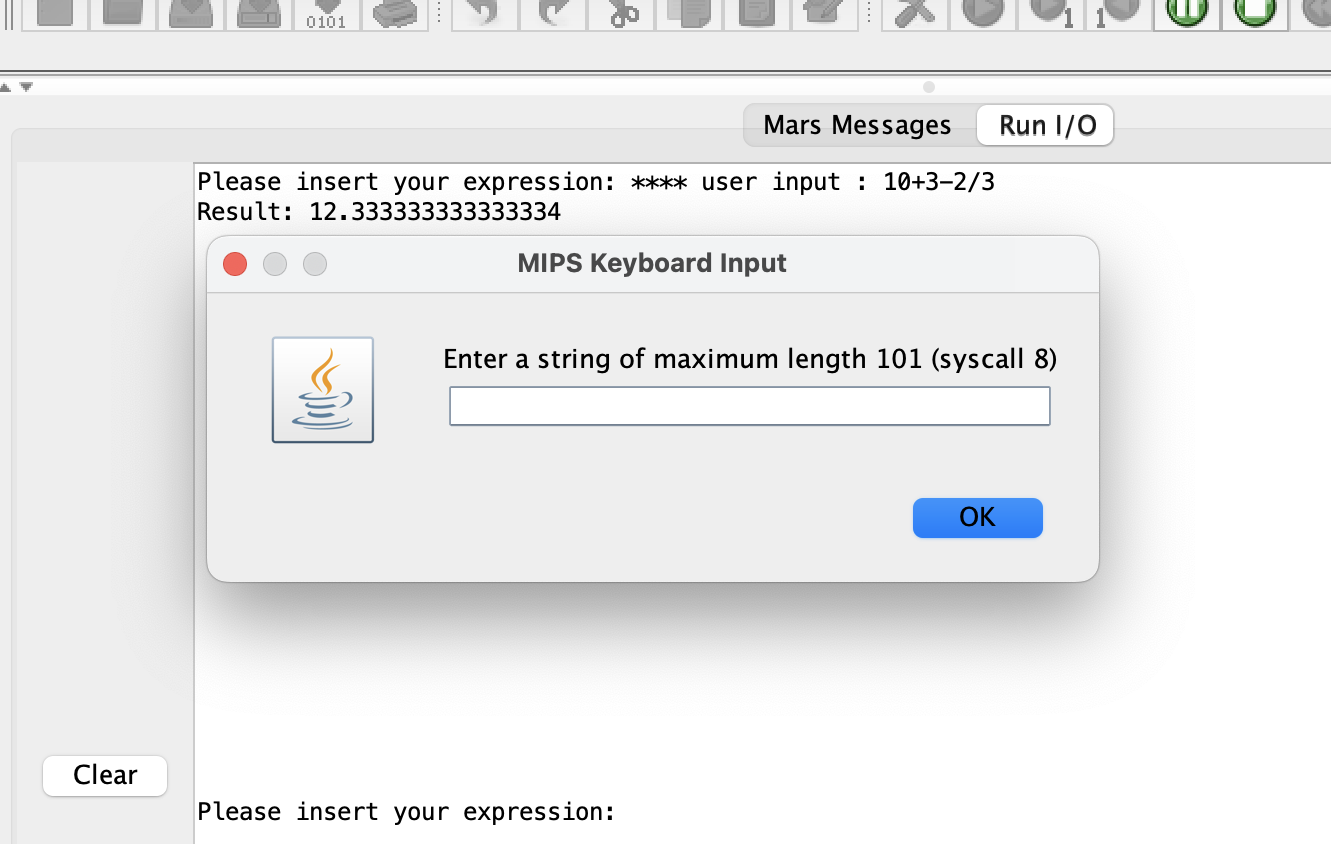
\includegraphics[width=0.6\textwidth]{graphics/1.Mars45Output.png}
        \caption{After entering the expression on \textit{Mars45}}
        \label{fig:1.MarsOutput}
    \end{figure}
    \section{Algorithm and Pseudo-code}

\label{2.Algorithm and PseudoCode}

I utilized Python code as a `\textit{pseudo-code}` for both MIPS32 Assembly and to validate algorithms. The following code section will be divided into three parts.

\subsection{Support Functions}
    The support functions below serve essential roles in facilitating the functionality of the main calculator algorithm.
    
    \begin{itemize}
        \item \textbf{fact(n: int) $\rightarrow$ int}: Calculating the factorial of \(n\). If \(n < 0\) or \(n > 16\), the function will raise an exception.
        
        \item \textbf{isOperand(char: str) $\rightarrow$ bool}: Checks if a character is an operand (numeric digit '0--9', decimal point '.', or memory indicator 'M').
        
        \item \textbf{isOperator(char: str) $\rightarrow$ bool}: Checks if a character is an operator (\(+\), \(-\), \(*\), \(/\), \(\hat{}\), \(!\)).
        
        \item \textbf{precedence(char: str) $\rightarrow$ int}: Determines the precedence of an operator.
    \end{itemize}
    
    These functions collectively contribute to properly parsing and evaluating mathematical expressions within the calculator program. The \texttt{fact} function computes factorials, ensuring the input is within acceptable bounds to prevent overflow. \texttt{isOperand} and \texttt{isOperator} ascertain whether a given character is an operand or an operator, respectively. Finally, \texttt{precedence} determines the precedence level of operators, aiding in correct expression evaluation.
        
    \begin{code}{Python}
        def fact(n: int) -> int:
            if n < 0:
                raise ValueError(f'Factorial of negative number, got n {n}')
            if n > 15:
                raise ValueError(f'Factorial of {n} is overflow in 32-bits')
            return 1 if n == 0 else n * fact(n - 1)
        
        def isOperand(char: str) -> bool:
            return char.isdigit() or char == '.' or char == 'M'
        
        def isOperator(char: str) -> bool:
            return char in ('+', '-', '*', '/', '^', '!')
        
        def precedence(char: str) -> int:
            if char == '+' or char == '-': return 1
            if char == '*' or char == '/': return 2
            if char == '^': return 3
            if char == '!': return 4
            return -1
    \end{code}
    \begin{lstlisting}[language=Python, caption=Support function in Python]
    \end{lstlisting}

\subsection{Converting Infix to Postfix Algorithm}
\label{sec:5.INFIX_TO_POSTFIX}
    The following Python code implements an algorithm to convert infix expressions to postfix notation   
    This algorithm scans the input expression character by character and applies specific rules to convert it to postfix notation. It handles operands, operators, and parentheses, and ensures the correct order of operations. Additionally, it accounts for negative numbers, unary minus, unary plus, and invalid characters, raising appropriate exceptions when encountered.
    
    \begin{code}{Python}
        def infixToPostfix(string: str, M: int):
            if len(string) == 0 or len(string) > 100:
                raise ValueError('Expression length must in range [0, 100], got length', len(string))
            
            stack: list[str] = []
            result: str = ''
            
            for char in string:
                if (isOperand(char)): result += char
                elif char == ' ': continue
                elif char == '(': stack.append(char)
                elif char == ')':
                    while stack and stack[-1] != '(': result += f' {stack.pop()}'
                    if stack and stack[-1] == '(': stack.pop()
                elif isOperator(char):
                    if char == '!':
                        result += ' !'
                        continue
                    
                    if (char == '-' 
                        and (not result or result[-1] in ('(', ' ', '*', '/', '^'))
                        and (not stack or stack[-1] in ('(', ' ', '*', '/', '^'))
                        ):
                        result += char
                        continue
                    
                    while (stack 
                           and stack[-1] != '(' 
                           and precedence(stack[-1]) >= precedence(char)):
                        result += f' {stack.pop()}'
                        
                    stack.append(char)
                    result += ' '
                else:
                    raise Exception('Invalid character')
        
            while stack: result += f' {stack.pop()}'
                
            return result
    \end{code}
    \begin{lstlisting}[language=Python, caption=Converting infix to postfix expression]
    \end{lstlisting}

\subsection{Evaluating Postfix Algorithm}
\label{sec:5.EVALUATE_POSTFIX}
    The following Python code implements an algorithm to evaluate postfix expressions.
    This algorithm iterates through the postfix expression, performing arithmetic operations and utilizing a stack to store intermediate results. It supports operands, operators, and memory variable 'M'. Additionally, it handles negative numbers and ensures proper expression evaluation. If the expression is invalid or cannot be evaluated, appropriate exceptions are raised.

    \begin{code}{Python}
        def evaluate_postfix(expression: str, M: int):
            stack: list[float] = []
            number: str = ''
        
            for char in expression:
                if char == 'M': 
                    number += str(M)
                elif isOperand(char) or (char == '-' and len(stack) < 2):
                    number += char
                elif char == ' ':
                    if number:
                        if number == '-':
                            stack.append(stack.pop() - operand2)
                            number = ''
                        else:
                            stack.append(float(number))
                            number = ''
                else:
                    if number:
                        stack.append(float(number))
                        number = ''
        
                    operand2 = stack.pop()
                    if char == '+':
                        stack.append(stack.pop() + operand2)
                    elif char == '-':
                        stack.append(stack.pop() - operand2)
                    elif char == '*':
                        stack.append(stack.pop() * operand2)
                    elif char == '/':
                        stack.append(stack.pop() / operand2)
                    elif char == '!':
                        stack.append(fact(int(operand2)))
                    elif char == '^':
                        operand2 = stack.pop()
                        stack.append(stack.pop() ** int(operand2))
                    else:
                        raise ValueError("Invalid token in expression")
            
            if number:
                stack.append(float(number))
        
            if len(stack) != 1:
                raise ValueError('Invalid postfix expression')
            
            return stack.pop()
    \end{code}
    \begin{lstlisting}[language=Python, caption=Evaluate Postfix]
    \end{lstlisting}
    \renewcommand{\arraystretch}{1.5}

\section{Description of Support Procedures}

\label{sec:3.SupportProcedures}

All procedures follow the convention of using \$a0-\$a3 as arguments and \$v0-\$v1 as return registers, taken from registers with smaller to larger values. All registers used by the procedures are stored in main memory, so when encountering the \texttt{jr \$ra} instruction, all registers are restored to their values before the subprocedure calculation.

For functions that need to use registers in Coprocessor 1 (\texttt{\$f<x>}), here is my convention for register management:

\begin{itemize}
    \label{sec:3.Coprocessor Management}
    \item \verb|Return|\space\space\space\space: \$f0 - \$f3
    \item \verb|Temporary|: \$f4 - \$f11
    \item \verb|Argument|\space\space: \$f12 - \$f15
    \item \verb|Temporary|: \$f16 - \$f19
    \item \verb|Constant|\space\space: \$f24 - \$f31
\end{itemize}

All privates prefixed with double underscores are indications of private procedures, only to be used within their own procedures or when called. The coder should not actively call them out.

\subsection{Description of character and string handling}
    The procedures below aid two main procedures, \texttt{INFIX\_TO\_POSTFIX} [\ref{sec:5.INFIX_TO_POSTFIX}] and \texttt{EVALUATE\_POSTFIX} [\ref{sec:5.EVALUATE_POSTFIX}], \texttt{STACK} [\ref{sec:4.Stack}], as well as other related procedures. They include character checks and string-handling functions
    
    \begin{longtable}{|m{2.5cm}|m{2.5cm}|m{2.5cm}|m{1cm}|m{5.6cm}|}
        \hline
            \textbf{Procedure} & 
            \textbf{Args} & 
            \textbf{Return} & 
            \centering \textbf{Leaf fucnt} &
            \textbf{Description}\\
        \hline
        \endfirsthead
            IS\_ OPERAND& 
            char = \$a0&
            bool = \$v0&
            \centering X&
            Checking if a character is an operand.\\
        \hline
            IS\_ OPERATOR& 
            char = \$a0&
            bool = \$v0&
            \centering X&
            Checking if a character is in (+, -, *, /, \^{}, !).\\
        \hline
            OPERATOR\_ PRECEDENCE& 
            char = \$a0&
            bool = \$v0&
            \centering X&
            Getting the precedence of an operator.\\
        \hline
            STRING\_ LENGTH& 
            str = \$a0&
            int = \$v0&
            \centering X&
            Getting the length of a string by looping through the string until it encounters the null or newline character. This procedure has a time complexity of \(O(n)\).\\
        \hline
            COMPARE\_ STRING& 
            str = \$a0
            \newline str = \$a1&
            bool = \$v0&
            &
            Comparing two strings by looping through both strings, return true if both strings are the same length and have identical contents. This operation has a time complexity of \(O(n)\).\\
        \hline
            RESET\_ STRING& 
            str = \$a0
            \newline str = \$a0&
            \centering void&
            \centering X&
            Resetting the space containing the string by looping through and replacing each character with a null character. This operation has a time complexity of \(O(n)\).\\
        \hline
        \caption{Description of Support Procedures} \\
    \end{longtable}

\subsection{Mathematics procedures}
    \begin{longtable}{|m{2.5cm}|m{2.5cm}|m{2.5cm}|m{1cm}|m{5.6cm}|}
        \hline
            \textbf{Procedure} & 
            \textbf{Args} & 
            \textbf{Return} & 
            \centering \textbf{Leaf fucnt} &
            \textbf{Description}\\
        \hline
        \endfirsthead
            FACTORIAL& 
            int = \$a0&
            int = \$v0&
            &
            Calculating the factorial of an integer using recursion. If the input is greater than 0 and less than 16, raise an exception and end the program. This operation has a time complexity of \(O(n)\).\\
        \hline
            EXPONENT& 
            double = \$f12
            \newline double = \$f14&
            double = \$f0&
            \centering X&
            Calculating the exponent of \$f12 \^{} \$f14 by looping. It automatically floors \$f14 into an integer and can calculate if \$f14 < 0.  This operation has a time complexity of \(O(|int(\$f14)|)\). Notice that if \$f12 = \$f14 = 0, raise an exception\\
        \hline
        \caption{Description of Mathematics Procedures} \\
    \end{longtable}

\subsection{Utility procedures}
    In this subsection, there will be utility procedures that do not contribute significantly to the algorithms of the \texttt{INFIX\_TO\_POSTFIX} [\ref{sec:5.INFIX_TO_POSTFIX}] and \texttt{EVALUATE\_POSTFIX} [\ref{sec:5.EVALUATE_POSTFIX}] procedures. They are used solely for display and assignment requirements.

    \begin{longtable}{|m{3.3cm}|m{2.9cm}|m{1.3cm}|m{1.1cm}|m{5.6cm}|}
        \hline
            \textbf{Procedure} & 
            \textbf{Args} & 
            \textbf{Return} & 
            \centering \textbf{Leaf fucnt} &
            \textbf{Description}\\
        \hline
        \endfirsthead
        \hline
            \textbf{Procedure} & 
            \textbf{Args} & 
            \textbf{Return} & 
            \centering \textbf{Leaf fucnt} &
            \textbf{Description}\\
        \hline
        \endhead
            END\_PROGRAM& 
            \centering -&
            void&
            \centering X&
            The exit prompt will be displayed, and the system call \$v0 = 10 will be invoked to end the program.\\
        \hline
            TYPE\_QUIT& 
            \centering -&
            void&
            \centering -&
            The quit prompt will be displayed, and the \texttt{END\_PROGRAM} procedure will be called.\\
        \hline
            WRITE\_ TO\_FILE& 
            message = \$a0 \newline filename = \$a1 \newline mode = \$a2&
            void&
            \centering -&
            This procedure is used to \emph{write} only with create (\$a2=1) or \emph{append} (\$a2=9) strings to a file. It automatically measures the length of the string to write to the file by calling the \texttt{STRING\_LENGTH} procedure and closes the file after writing to it.\\
        \hline
            new\_line& 
            \centering -&
            void&
            \centering X&
            When printing newline characters to the screen, note that this function will be convenient for code writers but will significantly slow down the program due to unnecessary procedures.\\
        \hline
        \caption{Description of Utility Procedures} \\
    \end{longtable}

    \newpage
    
    \subsubsection{Print Procedures}
        \label{sec:3.Print}
        The procedures below are considered leaf procedures supporting screen printing by calling \texttt{syscall}.
        
        \begin{multicols}{2}
            \begin{itemize}
                \label{sec:3.Print function}
                \item \verb|PRINT_DOUBLE|: double = \$f12
                \item \verb|PRINT_STRING|: string = \$a0
                \item \verb|PRINT_CHAR|\space\space\space: char = \$a0
                \item \verb|PRINT_INT|\space\space\space\space: int = \$a0
            \end{itemize}
        \end{multicols}

        Example:
        \begin{code}{ASM}
            # Integer
            li $a0, 2024
            jal PRINT_INT

            # Character
            li $a0, 97
            jal PRINT_CHAR

            # Double (The index of Coprocessor must be even)
            mov.d $f12, $f8 # Assume $f8 = 09052024.1259
            jal PRINT_DOUBLE
        \end{code}
        \begin{lstlisting}[language=ASM, caption=Color procedures]
        \end{lstlisting}
    
    \subsubsection{Color Procedures}
        \label{sec:3.Color}
        All procedures below are leaf procedures, simply using the \texttt{jal <COLOR LABEL>} command before and after a print command will suffice.
    
        \begin{multicols}{4}
            \begin{itemize}
                \item \verb|RED|
                \item \verb|GREEN|
                \item \verb|YELLOW|
                \item \verb|BLUE|
                \item \verb|MAGENTA|
                \item \verb|CYAN|
                \item \verb|RESET|
            \end{itemize}
        \end{multicols}
    
        Example:
        \begin{code}{ASM}
            jal CYAN
            la $a0, ascii_string # ascii_string: .asciiz "I'm studying CA at BKU\n"
            jal PRINT_STRING
            jal RESET
        \end{code}
        \begin{lstlisting}[language=ASM, caption=Color procedures]
        \end{lstlisting}
                
    \section{Stack Procedures}

\label{sec:4.Stack}

The following sub-section only discusses the design architecture of the Stack "\textit{class}", detailed explanations of the procedures will be covered further in the subsequent sub-sections.

\subsection{Stack Design Architecture}
    The Stack "\textit{class}" is designed by dividing a memory area \texttt{.space} into 3 parts. The first part holds the address of the word after the top of the stack, the next word is an integer indicating the number of elements inserted into the stack, and the remaining part is divided into word-sized regions containing the values of the elements pushed onto the stack [\ref{fig:4.StackArchitecture}]. If a Push operation exceeds the memory area, the system will report a stack overflow error, and if a \texttt{TOP} or \texttt{POP} operation is performed when the stack is empty, the system will report a stack underflow error.
    
    \begin{figure}[htbp]
        \centering
        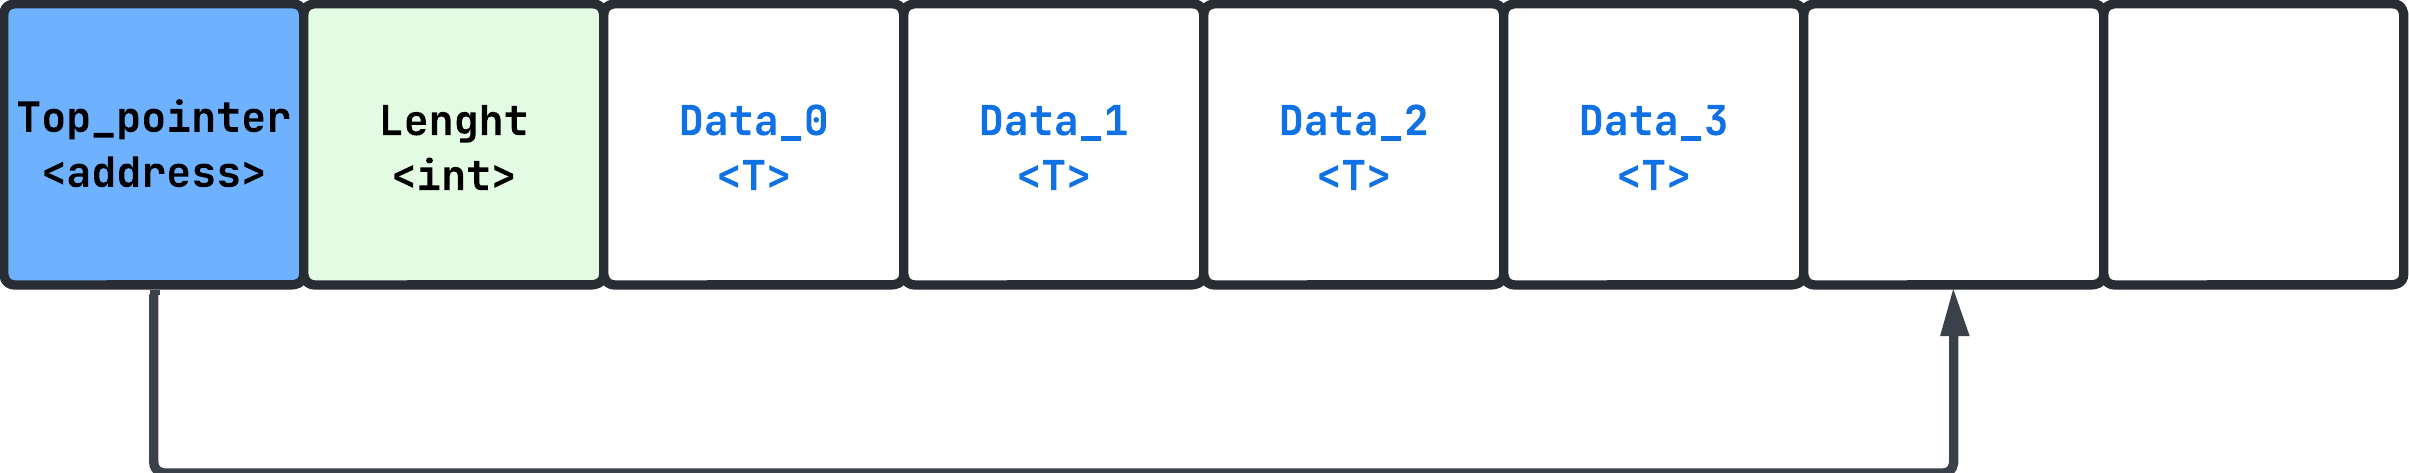
\includegraphics[width=1\textwidth]{graphics/3.StackArchitecture.png}
        \caption{Stack implementation architecture}
        \label{fig:4.StackArchitecture}
    \end{figure}
    
    An example of how data is organized in a stack:

    Let's push the each char \(HCMUT\) onto the stack sequentially. The result [\ref{fig:4.StackPrintMar}] shows that the first word at address \texttt{0x10010020} points to the address \texttt{0x1001003c}, meaning the word after the \texttt{TOP}.

    \begin{code}{ASM}
        la $a0, stack   # Load address of .space
        
        # STACK_PUSH($a0 = address of memory block, $a1 = value) => void
        li $a1, H
        jal STACK_PUSH
        li $a1, C
        jal STACK_PUSH
        li $a1, M
        jal STACK_PUSH
        li $a1, U
        jal STACK_PUSH
        li $a1, T
        jal STACK_PUSH
        
        la $a1, PRINT_CHAR
        jal PRINT_STACK
    \end{code}

\begin{figure}[htbp]
    \centering
    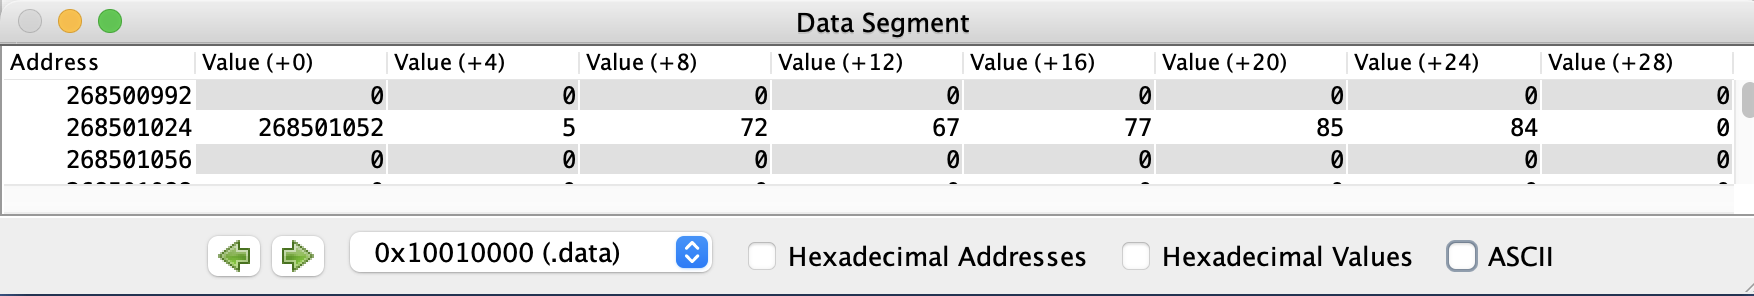
\includegraphics[width=1\textwidth]{graphics/3.StackPrintMar.png}
    \caption{Stack memory architecture}
    \label{fig:4.StackPrintMar}
\end{figure}

\subsection{Stack Procedures API}
    This sub-section contains all the MIPS32 procedures API for the Stack "\textit{class}". All procedures below use register \texttt{\$a0} to pass the address of the memory block containing the address of the \texttt{Top\_pointer} (the blue block in figure [\ref{fig:4.StackArchitecture}]). All procedures have time complexity of \(O(1)\), except \texttt{STACK\_RESET} and \texttt{STACK\_PRINT} have complexity of \(O(n)\).

    \begin{longtable}{|m{3cm}|m{3cm}|m{2cm}|m{1cm}|m{5.1cm}|}
        \hline
            \textbf{Procedure} & 
            \textbf{Args} \newline (\texttt{\$a0} = \textit{memory block address}) & 
            \textbf{Return} & 
            \centering \textbf{Leaf fucnt} &
            \textbf{Description}\\
        \hline
        \endfirsthead
        \hline
            \textbf{Procedure} & 
            \textbf{Args} \newline (\texttt{\$a0} = \textit{memory block address}) & 
            \textbf{Return} & 
            \centering \textbf{Leaf fucnt} &
            \textbf{Description}\\
        \hline
        \endhead
            STACK\_INIT& 
            \centering -&
            void&
            \centering X&
            This procedure \textbf{MUST} be called before using a block of memory as a stack in other to set up the \texttt{Top\_pointer}\\
        \hline
            STACK\_ LENGTH& 
            \centering -&
            int = \$v0&
            \centering X&
            Return the number of elements in the stack.\\
        \hline
            STACK\_PUSH& 
            <T> = \$a1&
            void&
            &
            Adding the element at the end of the stack.\\
        \hline
            STACK\_TOP& 
            \centering -&
            <T> = \$v0&
            &
            Return the value of the last element of the stack\\
        \hline
            STACK\_POP& 
            \centering -&
            <T> = \$v0&
            &
            Removing and returning the last element of the stack.\\
        \hline
            STACK\_ PUSH\_DOUBLE& 
            double = \$f12&
            void&
            &
            Adding the double values \$f12 and \$f13 in this order into the stack.\\
        \hline
            STACK\_POP\_ DOUBLE& 
            \centering -&
            double = \$f0 = \$v0&
            &
            Removing and returning the last double value of the stack.\\
        \hline
            STACK\_ LENGTH\_ DOUBLE& 
            \centering -&
            int = \$v0&
            &
            Return the length of the stack containing double by calling \texttt{STACK\_LENGTH} and dividing by 2 the values it returns.\\
        \hline
            STACK\_ RESET&
            \centering -&
            void&
            \centering X&
            Pop all elements in stack and reset \texttt{Top\_pointer} and \texttt{Length}.\\
        \hline
            PRINT\_STACK& 
            print func = \$a1 \newline [\ref{sec:3.Print function}]&
            void&
            &
            Print all stack properties. The format for displaying on the screen will be: \newline \texttt{|\textit{X}|\textit{X}|\textit{X}|<-TOP (Length=\textit{Y})}\\
        \hline
        \caption{Description of Stack Procedures}\\
    \end{longtable}

    \subsection{Stack Exception Handling}
        The procedures below are private and will be automatically called when an error occurs.
    
        \begin{longtable}{|m{7.5cm}|m{7.5cm}|}
            \hline
                \textbf{Private Exception} & 
                \textbf{Description}\\
            \hline
            \endfirsthead
            \hline
                \textbf{Private Exception} & 
                \textbf{Description}\\
            \hline
            \endhead
                \_\_STACK\_OVERFLOW& 
                \_\_STACK\_OVERFLOW will be called when \texttt{Push} more than 25 doubles or 50 other elements into the stack. This involves printing an error message and exiting the program.\\
            \hline
                \_\_STACK\_OVERFLOW&
                \_\_STACK\_OVERFLOW will be called when \texttt{Pop} or \texttt{Top} an empty stack. This involves printing an error message and exiting the program.\\
            \hline
            \caption{Description of Stack Exception}\\
        \end{longtable}
    \section{Limitations}
    In this section, I will outline areas where the program can be further improved in the future. These areas are listed from \textbf{\textit{major issues to minor ones}}.
    
    \subsection{Handling Unary Operations}
        My program still has numerous bugs, especially in handling unary operations such as addition and minus. I've tested several cases like multiple consecutive addition or subtraction signs before a number, or a minus sign before a parenthesis, and the program crashes. This occurs due to flaws in my Python algorithm. The following code is the result of both MIPS32 and Python.

        \label{sec:5.Limitations}
        \begin{code}{bash}
            >>> Please insert your expression: -1*-(3+1)
            >>> Result: 2
            >>>
            >>> Please insert your expression: (-1)*(-1)-1*-1
            >>> Error: Invalid postfix expression
            >>> Result: -0
            >>> 
            >>> Please insert your expression: -1--2
            >>> Error: Invalid postfix expression
            >>> Result: -2
            >>> 
            >>> Please insert your expression: -1+-2
            >>> PROGRAM IS CRACKING
            >>> 
            >>> Please insert your expression: 1++++++2
            >>> PROGRAM IS CRACKING
            >>> 
            >>> Please insert your expression: -1*(3+1
            >>> PROGRAM IS CRACKING
        \end{code}
        \begin{lstlisting}[language=bash, caption={Failing testcase}]
        \end{lstlisting}
    
    \subsection{Error Handling}
        I haven't implemented error handling yet. The program usually freezes [\ref{sec:5.Limitations}] instead of automatically resetting and restarting the program from the beginning when an error occurs.
    
    \subsection{Arithmetic Overflow Causing File Output Error}
        Although the program still produces approximately correct results when computing with large numbers, when exporting the result to a file, it outputs strange characters. This is because there are still many issues with my \texttt{DOUBLE\_TO\_STRING} procedure. An example for this issue:

        \begin{code}{bash}
            >>> Please insert your expression: 10^100
            >>> Result: 1.0000000000000006e+100
            In calc_log.txt: 
                -./,),(-*,(../,),(-*,(./,),(-*,(
        \end{code}
        \begin{lstlisting}[language=bash, caption={Wrong result in \textit{.txt} file}]
        \end{lstlisting}

    \subsection{String Class Design}
        I haven't designed a "class" for strings like I did for the "stack" because I had already written string processing functions. Consequently, these procedures all have a complexity of \(O(n)\).
    
    \subsection{Usage of Load and Store Commands}
        When coding subprocedures, I always use the \texttt{sw} and \texttt{lw} commands for all \texttt{\$a<x>} and \texttt{\$t<x>} registers to make the code and debugging easier. As the theoretical class mentions, \texttt{lw} and \texttt{sw} commands consume more time than other commands. This leads to the excessive use of subprocedures for easier coding and debugging but at the cost of reducing the program's speed.
    
    \subsection{Heap Memory Usage}
        I don't utilize heap memory for allocation; instead, I only use the main memory (stack) for this purpose. Consequently, my program cannot handle cases with excessively large or numerous numbers while running.
    
    
    \bibliographystyle{plainnat}
    \bibliography{refs.bib}
    \addbibresource{refs.bib}
    \nocite{*}
\end{document}